%%This is a very basic article template.
%%There is just one section and two subsections.
\documentclass[a4paper]{jarticle}
\title{人生調和振動子}
\author{したろう}
\date{}
%%<Preamble>
%パッケージ
\usepackage[dvipdfmx]{graphicx, color}		%画像処理
\usepackage{amssymb}
\usepackage{amsmath}
\usepackage{bm}
\usepackage{ascmac} 
\usepackage{theorem}
\usepackage{fancybox} 
\usepackage{cases}
\usepackage{subfigure}
\usepackage{listings}
\pagestyle{myheadings}		%ページ番号なし
\usepackage[cmbtt]{bold-extra}  % CMフォントのタイプライター体のボールドを使う
% listingsパッケージのデフォルトを設定する
\lstset{%
  language={Python},             % 言語をCにする
  basicstyle={\ttfamily},   % プログラムの基本スタイルは等幅(tt)とする
  keywordstyle={\bfseries}, % 予約語は太字(bf)にする
  numbers=left,             % 左側に行番号を入れる
  frame=single,             % 枠で囲む
  lineskip=-0.75ex,         % プログラムリストの改行幅を少し小さくする
  captionpos=b              % キャプションの位置をプログラムの下にする
}
%余白の定義
\newlength{\topdummy}
\setlength{\topdummy}{\topmargin}
\setlength{\topmargin}{-2cm}
\setlength{\oddsidemargin}{-0.5cm}
\setlength{\evensidemargin}{-0.5cm}
\setlength{\footskip}{-0.5cm}
\addtolength{\textheight}{\topdummy}
\addtolength{\textheight}{-\topmargin}
\addtolength{\textheight}{1.5cm}
\setlength{\textwidth}{\paperwidth}
\addtolength{\textwidth}{-\evensidemargin}
\addtolength{\textwidth}{-\oddsidemargin}
\addtolength{\textwidth}{-5.0cm}
%%</Preamble>
%%<macro>
\def\Arg{\mathrm{Arg}} %偏角
\def\arwvc#1{\overrightarrow{\mathrm{#1}}}	%矢印ベクトル表示
\def\Vec#1{\mbox{\boldmath $#1$}}	
%太字でイタリック体のまま太字にする(テキストモード,数式モードのいずれにおいても使用可能)
\def\Bar#1{\overline{#1}}	%複素共役
\def\dps{\displaystyle}		%"\displaystyle"の省略
\def\df#1#2{\frac{\mathrm{d} #1}{\mathrm{d} #2}}		%微分の省略
\def\pd#1#2{\frac{\partial #1}{\partial #2}}		%偏微分の省略
\def\unit#1{\ \mathrm{#1}}		%単位
\def\deg{{{}^\circ}}		%摂氏記号の省略
\def\epsilon{\varepsilon}	%イプシロンをεに統一
\def\grad{\mathrm{grad}}	%グラディエント
\def\div{\mathrm{div}}		%ダイバージェンス
\def\rot{\mathrm{rot}}		%ローテーション
\def\mr#1{\mathrm{#1}}	%数式モードでのローマン体入力
\def\dint#1#2#3{\int_{#1}^{#2}\mathrm{d}#3}	%定積分
\def\atom#1#2{${}^{#2}\mathrm{#1}$}
\def\<{\langle}
\def\>{\rangle}
%%</macro>
\begin{document}
\maketitle
\section{概要}
単振動とは一定の周期で行う往復運動である.
単振動は簡単なモデルとして物理学の枠組みを超えて
様々なところに現れる.
本稿では人生に対しても同様の単振動が見られることを考察する.

\section{原理}
\subsection{単振動}
微分方程式
\begin{align}
	\df{^2}{t^2} x(t)
	+
	\omega^2 x^2
	=
	0
	\label{eq}
\end{align}
で表される運動が単振動である.
微分方程式(\ref{eq})の解を図\ref{fig}
で表す.
\begin{figure}[htbp]
	\begin{center}
		% GNUPLOT: LaTeX picture with Postscript
\begingroup
  \makeatletter
  \providecommand\color[2][]{%
    \GenericError{(gnuplot) \space\space\space\@spaces}{%
      Package color not loaded in conjunction with
      terminal option `colourtext'%
    }{See the gnuplot documentation for explanation.%
    }{Either use 'blacktext' in gnuplot or load the package
      color.sty in LaTeX.}%
    \renewcommand\color[2][]{}%
  }%
  \providecommand\includegraphics[2][]{%
    \GenericError{(gnuplot) \space\space\space\@spaces}{%
      Package graphicx or graphics not loaded%
    }{See the gnuplot documentation for explanation.%
    }{The gnuplot epslatex terminal needs graphicx.sty or graphics.sty.}%
    \renewcommand\includegraphics[2][]{}%
  }%
  \providecommand\rotatebox[2]{#2}%
  \@ifundefined{ifGPcolor}{%
    \newif\ifGPcolor
    \GPcolortrue
  }{}%
  \@ifundefined{ifGPblacktext}{%
    \newif\ifGPblacktext
    \GPblacktexttrue
  }{}%
  % define a \g@addto@macro without @ in the name:
  \let\gplgaddtomacro\g@addto@macro
  % define empty templates for all commands taking text:
  \gdef\gplbacktext{}%
  \gdef\gplfronttext{}%
  \makeatother
  \ifGPblacktext
    % no textcolor at all
    \def\colorrgb#1{}%
    \def\colorgray#1{}%
  \else
    % gray or color?
    \ifGPcolor
      \def\colorrgb#1{\color[rgb]{#1}}%
      \def\colorgray#1{\color[gray]{#1}}%
      \expandafter\def\csname LTw\endcsname{\color{white}}%
      \expandafter\def\csname LTb\endcsname{\color{black}}%
      \expandafter\def\csname LTa\endcsname{\color{black}}%
      \expandafter\def\csname LT0\endcsname{\color[rgb]{1,0,0}}%
      \expandafter\def\csname LT1\endcsname{\color[rgb]{0,1,0}}%
      \expandafter\def\csname LT2\endcsname{\color[rgb]{0,0,1}}%
      \expandafter\def\csname LT3\endcsname{\color[rgb]{1,0,1}}%
      \expandafter\def\csname LT4\endcsname{\color[rgb]{0,1,1}}%
      \expandafter\def\csname LT5\endcsname{\color[rgb]{1,1,0}}%
      \expandafter\def\csname LT6\endcsname{\color[rgb]{0,0,0}}%
      \expandafter\def\csname LT7\endcsname{\color[rgb]{1,0.3,0}}%
      \expandafter\def\csname LT8\endcsname{\color[rgb]{0.5,0.5,0.5}}%
    \else
      % gray
      \def\colorrgb#1{\color{black}}%
      \def\colorgray#1{\color[gray]{#1}}%
      \expandafter\def\csname LTw\endcsname{\color{white}}%
      \expandafter\def\csname LTb\endcsname{\color{black}}%
      \expandafter\def\csname LTa\endcsname{\color{black}}%
      \expandafter\def\csname LT0\endcsname{\color{black}}%
      \expandafter\def\csname LT1\endcsname{\color{black}}%
      \expandafter\def\csname LT2\endcsname{\color{black}}%
      \expandafter\def\csname LT3\endcsname{\color{black}}%
      \expandafter\def\csname LT4\endcsname{\color{black}}%
      \expandafter\def\csname LT5\endcsname{\color{black}}%
      \expandafter\def\csname LT6\endcsname{\color{black}}%
      \expandafter\def\csname LT7\endcsname{\color{black}}%
      \expandafter\def\csname LT8\endcsname{\color{black}}%
    \fi
  \fi
  \setlength{\unitlength}{0.0500bp}%
  \begin{picture}(7200.00,5040.00)%
    \gplgaddtomacro\gplbacktext{%
      \csname LTb\endcsname%
      \put(946,704){\makebox(0,0)[r]{\strut{}-1}}%
      \put(946,1722){\makebox(0,0)[r]{\strut{}-0.5}}%
      \put(946,2740){\makebox(0,0)[r]{\strut{} 0}}%
      \put(946,3757){\makebox(0,0)[r]{\strut{} 0.5}}%
      \put(946,4775){\makebox(0,0)[r]{\strut{} 1}}%
      \put(1078,484){\makebox(0,0){\strut{}0}}%
	  \put(2509,484){\makebox(0,0){\strut{}$\frac{\pi}{2}$}}%
      \put(3941,484){\makebox(0,0){\strut{}$\pi$}}%
	  \put(5372,484){\makebox(0,0){\strut{}$\frac{3}{2}\pi$}}%
      \put(6803,484){\makebox(0,0){\strut{}$2\pi$}}%
	  \put(176,2739){\rotatebox{-270}{\makebox(0,0){\strut{}Happy $\unit{(J)}$}}}%
	  \put(3940,154){\makebox(0,0){\strut{}Time$\unit{(yr)}$}}%
    }%
    \gplgaddtomacro\gplfronttext{%
      \csname LTb\endcsname%
      \put(5816,4602){\makebox(0,0)[r]{\strut{}$y=\sin x$}}%
    }%
    \gplbacktext
    \put(0,0){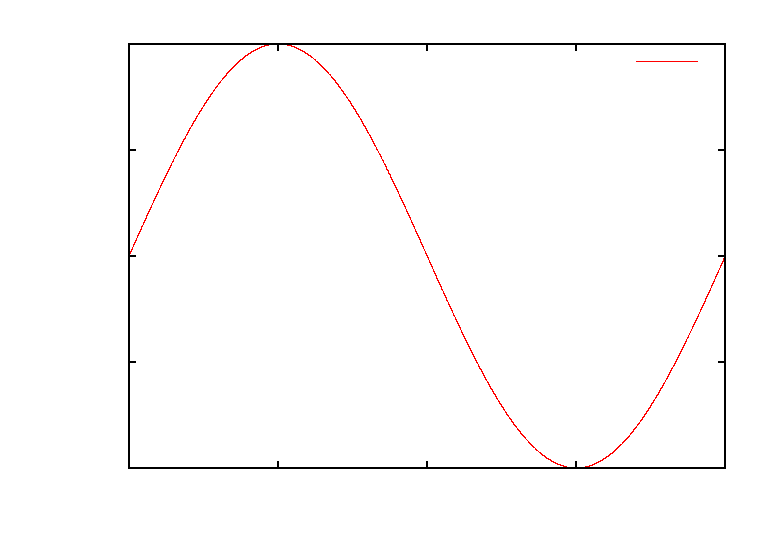
\includegraphics{sin}}%
    \gplfronttext
  \end{picture}%
\endgroup

		\label{fig}
		\caption{これが人生}
	\end{center}
\end{figure}

\newpage
\begin{thebibliography}{9}
	\bibitem{text}
		国立天文台,『理科年表 平成27年』丸善出版,2014.
\end{thebibliography}

\end{document}
